%!TEX root = ../thesis.tex

\chapter{Deep neural networks for predicting DNA methylation}

% **************************** Define Graphics Path **************************
\ifpdf
    \graphicspath{{Chapter4/Figs/Raster/}{Chapter4/Figs/PDF/}{Chapter4/Figs/}}
\else
    \graphicspath{{Chapter4/Figs/Vector/}{Chapter4/Figs/}}
\fi

\begin{figure}[htbp!]
\centering
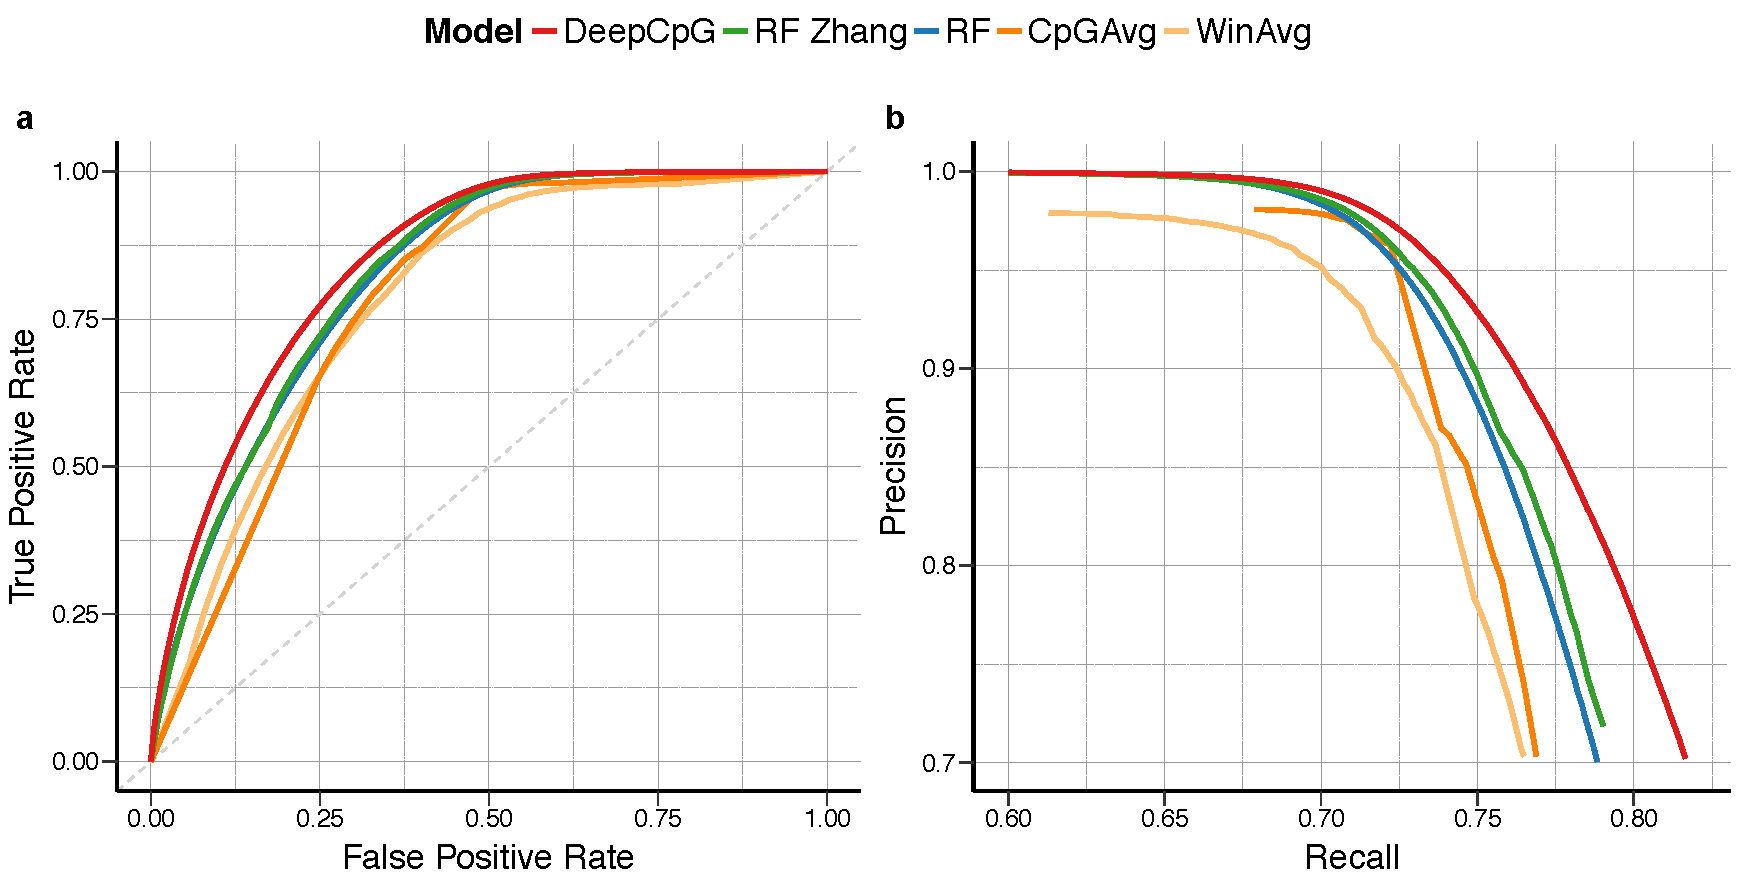
\includegraphics[width=1.0\textwidth]{curves}
\caption[Receiver operating characteristic and precision recall curves for predicting DNA methylation states using alternative methods.]{Receiver operating characteristic and precision recall curves for predicting DNA methylation states using alternative methods. Receiver operating characterisic curve (a) and precision recall curve (b) for predicting methylation states in serum ESCs, analogous to results shown in main Figure 2. Considered were DeepCpG and random forest classifiers, either trained using similar features as DeepCpG (RF) or using additional DNA annotations (RF Zhang). Two baseline methods were considered, which estimate methylation states by averaging observed methylation states, either across consecutive 3 kb regions within individual cells (WinAvg), or across cells at a single CpG site (CpGAvg). Curves represent the average performance across cells.}
\label{fig:dcpg_eval_curves}
\end{figure}

\begin{figure}[htbp!]
\centering
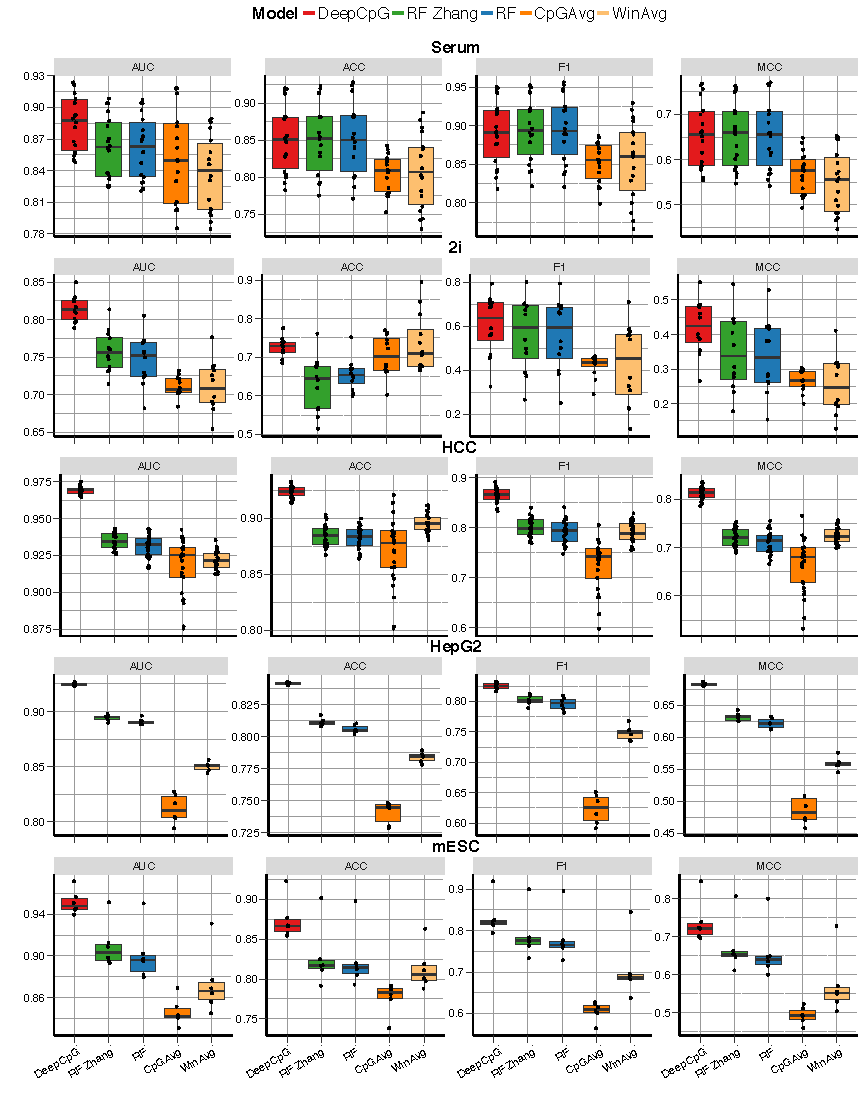
\includegraphics[width=1.0\textwidth]{dsets}
\caption[Prediction performance of alternative methods and metrics across five datasets.]{Prediction performance of alternative methods and metrics across five datasets. Test prediction performance metrics for 18 serum and 12 2i mouse ESCs profiled using scBS-seq, as well as for cells profiled using scRRBS-seq, including 25 human HCC cells, 6 HepG2 cells, and 6 additional mouse ESCs. Shown is the prediction performance for alternative methods, considering the area under receiver operating characteristic curve (AUC), accuracy (ACC), F1 score (F1), or Matthews correlation coefficient (MCC).}
\label{fig:dcpg_eval_dsets_all}
\end{figure}

\begin{figure}[htbp!]
\centering
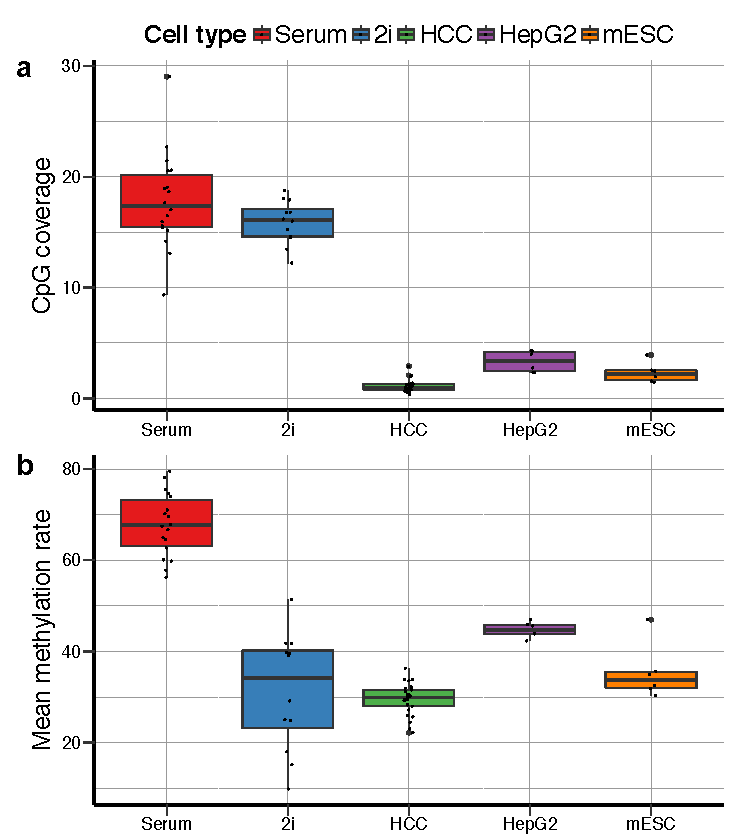
\includegraphics[width=0.7\textwidth]{cells}
\caption[Quality metrics of cells profiled using scBS-seq and scRRBS-seq.]{Quality metrics of cells profiled using scBS-seq and scRRBS-seq. Genome wide CpG coverage (a) and mean methylation rate (b) of cells profiled using scBS-seq (Serum, 2i), and scRRBS-seq (HCC, HepG2, mESC).}
\label{fig:dcpg_eval_cells}
\end{figure}

\begin{figure}[htbp!]
\centering
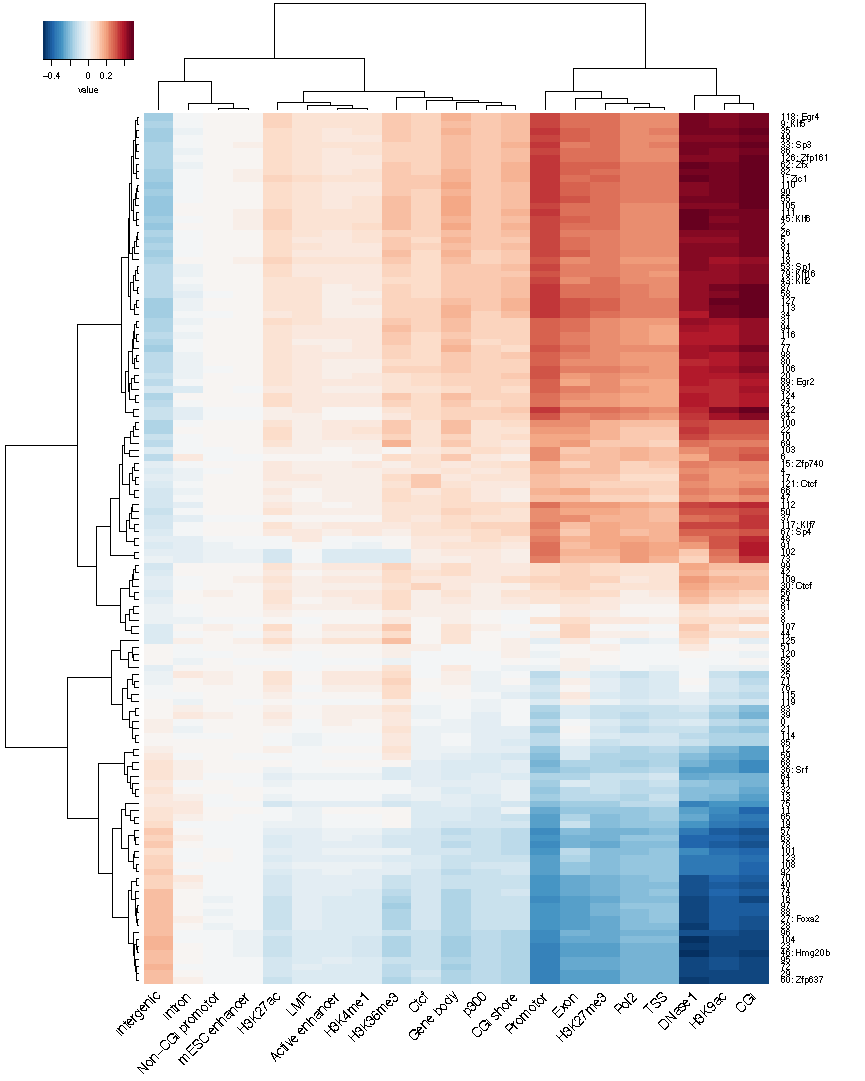
\includegraphics[width=1.0\textwidth]{motifs_feat}
\caption[Correlation between filter activities and higher-level sequence features.]{Correlation between filter activities and higher-level sequence features. Spearman correlation between the activity of filters of the first convolutional layer of the DNA module (motifs) and higher-level sequence features considered in Zhang et al. Activities were strongly correlated with DNase1 hypersensitive sites, histone modification marks, and CpG dense genomic context. This indicates that DeepCpG is able to automatically learn higher-level features from the raw DNA sequence.}
\label{fig:dcpg_eval_motifs_feat}
\end{figure}

\begin{figure}[htbp!]
\centering
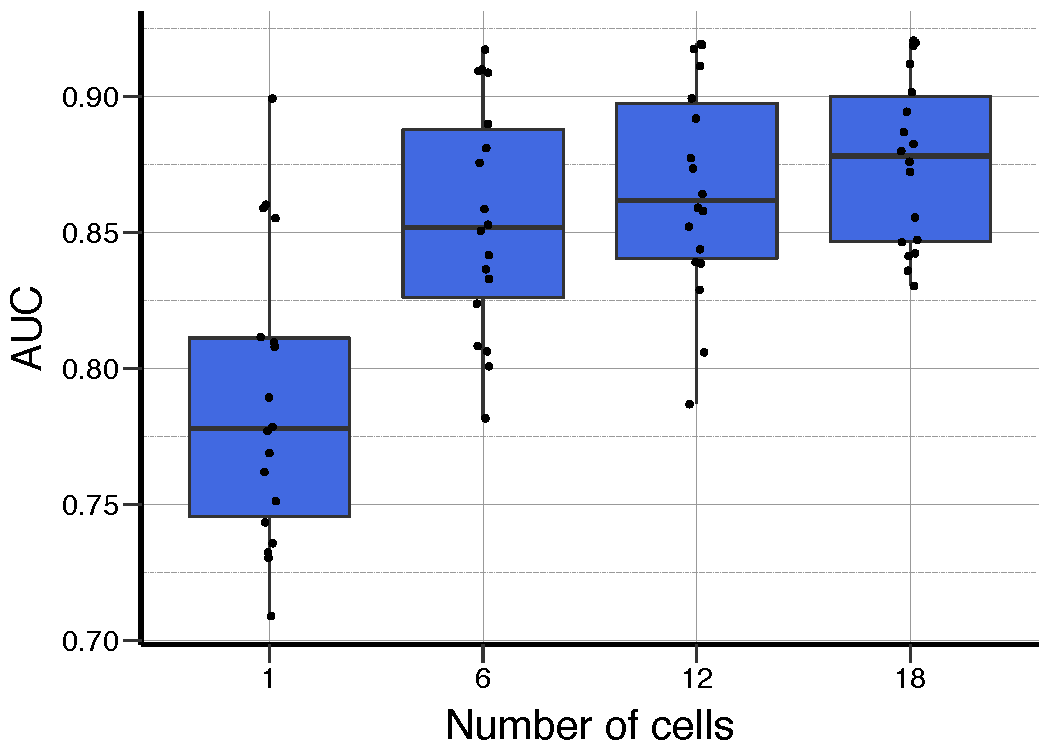
\includegraphics[width=0.6\textwidth]{cpg_module}
\caption[Prediction performance of the DeepCpG CpG module depending on the number of cells.]{Prediction performance of the DeepCpG CpG module depending on the number of cells. Test AUC for serum mouse ESCs, using an increasing number of cells as input for the DeepCpG CpG module.}
\label{fig:dcpg_eval_cpg_module}
\end{figure}

\begin{figure}[htbp!]
\centering
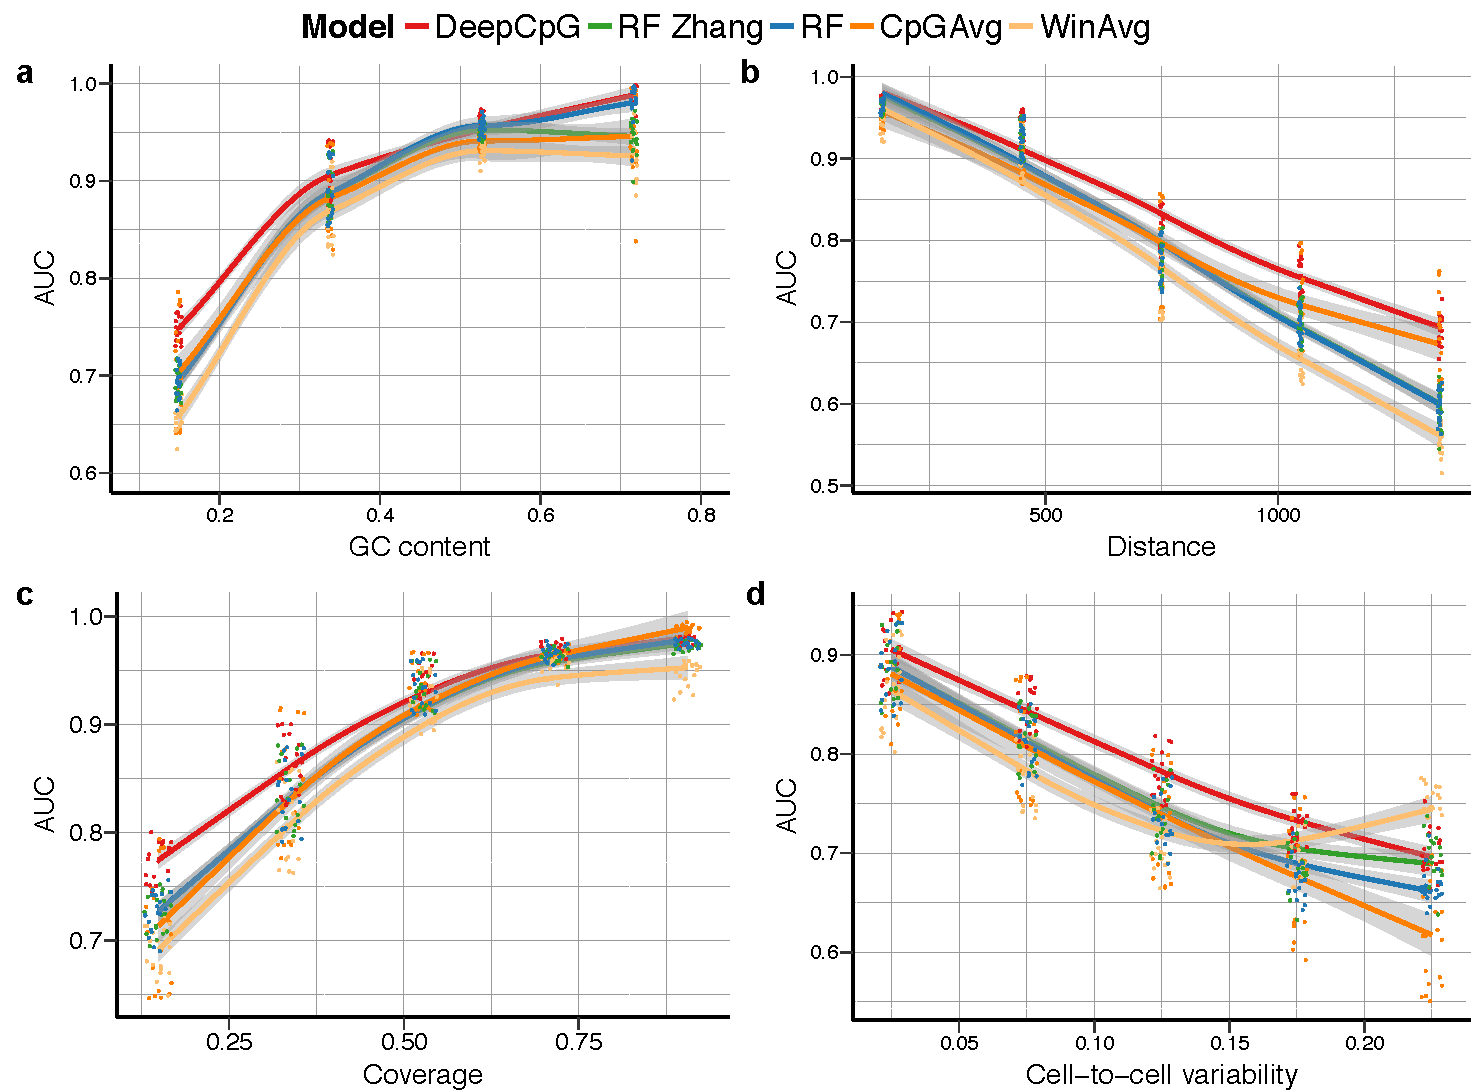
\includegraphics[width=1.0\textwidth]{stats}
\caption[Prediction performances stratified by different metrics.]{Prediction performances stratified by different metrics. Test AUC for serum mouse ESCs, considering alternative methods, stratified by (a) GC content, (b) distance to neighboring CpG sites, (c) fraction of cells by which the target CpG site is covered, (d) cell-to-cell variability within 3 kb windows centered on the target CpG site. Trend lines were fit to observed coverage levels using local polynomial regression (LOESS), with shaded areas corresponding to 95\% confidence intervals.}
\label{fig:dcpg_eval_stats}
\end{figure}
